\documentclass[../TG_magistrsko_delo_sections.tex]{subfiles}
\graphicspath{{\subfix{../images/}}}

\begin{document}
Daljši in bolj zapleten del dokaza izreka Šarkovskega je za nami. Sedaj moramo dokazati še drugi del, ki pravi:
\begin{izrek}
Vsak rep $\mathcal{T}$ ureditve Šarkovskega je množica period za neko zvezno funkcijo $f$, ki slika interval nazaj vase.
\end{izrek}
\begin{proof}
Izrek bomo dokazali tako, da bomo za vsak rep $\mathcal{T}$ poiskali funkcijo, katere množica period je enaka repu $\mathcal{T}$. Pri iskanju primerne funkcije si bomo pomagali z družino odrezanih šotorskih funkcij:
\begin{equation*} %\label{eq1}
\begin{split}
T_h &:  [0, 1] \to [0, 1] \\ 
T_h &: x \mapsto \min \left(h, 1- 2 \left|x-\frac{1}{2} \right|\right)
\end{split}
\end{equation*}
Ekvivalentno in mogoče lažje predstavljivo lahko predpis funkcije $T_h$ zapišemo na naslednji način:
\begin{equation*} %\label{eq1}
T_h(x) = \min(2x, 2-2x, h).
\end{equation*}
Točke, ki imajo za funkcijo $T_h$ periodo $n$, so negibne točke za funkcijo $T_h^n$, zato si zaradi lažje predstave na sliki~\ref{fig:Th} ogledamo funkcije $T_{0,85}, T_{0,85}^2, T_{0,85}^3$ in $T_{0,85}^4$. 
\begin{figure}[h]
  \centering
  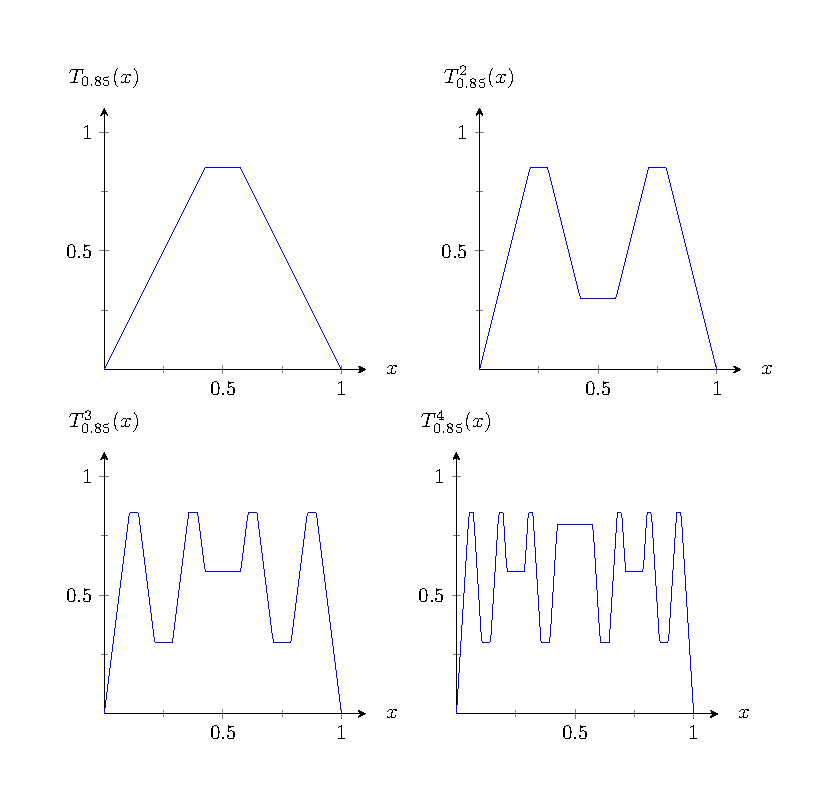
\includegraphics{odrezana_funkcija.pdf}
% \caption[caption za v kazalo]{Dolg caption pod sliko}
  \caption[Primer vektorske slike.]{Funkcije  $T_{0,85}, T_{0,85}^2, T_{0,85}^3$ in $T_{0,85}^4$ in njihova presečišča s simetralo lihih kvadrantov.}
  \label{fig:Th}
\end{figure}

V nadaljevanju dokaza bo zelo pomembna funkcija $T_1$. Na sliki~\ref{fig:T1} so prikazane prve štiri iteracije funkcije $T_1$. S slike razberemo, da ima funkcija $T_1$ dve presečišči s simetralo lihih kvadrantov in zato tudi dve negibni točki. Funkcija $T_1^2$ ima 4 negibne točke, funkcija $T_1^3$ jih ima 8, funkcija $T_1^4$ pa 16. Ugotovimo, da funkcija $T_1^n$ seka simetralo lihih kvadrantov natanko $2^n$-krat in ima prav toliko negibnih točk. Funkcija $T_1$ pa ima po tem razmisleku največ $2^n$ točk s periodo $n$.
\begin{figure}[h]
  \centering
  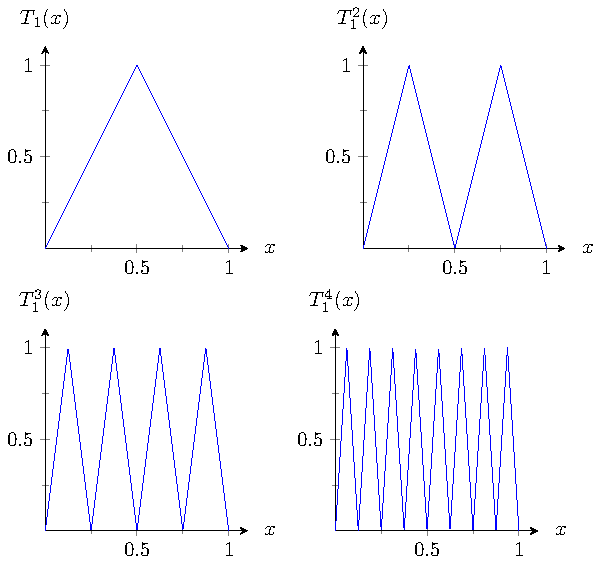
\includegraphics{funkcija_T1.pdf}
% \caption[caption za v kazalo]{Dolg caption pod sliko}
  \caption[Primer vektorske slike.]{Funkcije $T_1, T_1^2, T_1^3, T_1^4$ in njihova presečišča s simetralo lihih kvadrantov.}
  \label{fig:T1}
\end{figure}

Za dokaz izreka bomo najprej pokazali, da obstaja funkcija, ki ima samo periodo 1. To je funkcija $T_0$. Za vsak $x \in [0, 1]$ je vrednost funkcije $T_0$ enaka 0, zato je 0 tudi edina periodična točka za to funkcijo. Točka 0 je negibna točka, zato je njena perioda enaka 1.

Obravnavajmo funkcijo $T_1$. Dokazali bomo, da je vsako naravno število $n$ perioda funkcije $T_1$. To najlažje dokažemo tako, da poiščemo cikel dolžine 3 in s pomočjo izreka~\ref{izr:forcing} sklepamo, da ima funkcija $T_1$ vse periode. Vsaka točka ki ima za funkcijo $T_1$ periodo 3 je negibna točka funkcije $T_1^3$, zato si poglejmo negibne točke funkcije $T_1^3$. Iz grafa razberemo, da ima funkcija $T_1^3$ osem negibnih točk. Izračunamo lahko, da sta točki 0 in $\frac{2}{3}$ sta negibni točki funkcije $T_1$, točke $\frac{2}{7}, \frac{4}{7}$ in $\frac{6}{7}$ tvorijo 3-cikel. Prav tako tvorijo 3-cikel točke  $\frac{2}{9}, \frac{4}{9}$ in $\frac{8}{9}$. S pomočjo izreka~\ref{izr:forcing} ugotovimo, da funkcija $T_1$ vsebuje točke vseh period, saj vsebuje točko periode 3.

Funkciji $T_1$ in $T_h$ sta vsaj na nekem delu intervala $[0, 1]$ enaki, zato lahko pričakujemo, da obstajajo cikli, ki so skupni obema funkcijama. O tem govori naslednja lema:
\begin{lema}\label{lem:t1th}
Za funkciji $T_1$, $T_h$ in njune cikle  veljata naslednji dve trditvi:
\begin{enumerate}[label={(\arabic*)}]
\item Če je $\mathcal{O} \subseteq [0, h]$ cikel za funkcijo $T_1$, je tudi cikel za funkcijo $T_h$. \label{trd:t1toth}
\item Če je $\mathcal{O} \subseteq [0, h)$ cikel za funkcijo $T_h$, je cikel tudi za funkcijo $T_1$. \label{trd:thtot1}
\end{enumerate}
\end{lema}
\begin{proof}
Funkciji $T_1$ in $T_h$ se razlikujeta samo v tistih točkah $x$, za katere je $T_1(x) > h$. V vseh ostalih točkah, sta funkciji enaki. Privzemimo, da je $\mathcal{O} \subseteq [0, h]$ cikel za funkcijo $T_1$. Ker je cikel $\mathcal{O}$ vsebovan v intervalu $[0, h]$, za vsako točko $x \in \mathcal{O}$ velja $T_1(x) \leq h$. Torej velja $T_1(x)=T_h(x)$, kar pomeni, da je $\mathcal{O}$ tudi cikel za funkcijo $T_h$. Dokazali smo trditev~\ref{trd:t1toth}

Za dokaz trditve~\ref{trd:thtot1} prespostavimo, da je $\mathcal{O} \subseteq [0, h)$ cikel za funkcijo $T_h$. Torej je za vsako točko $x$ iz cikla $\mathcal{O}$ slika $T_h(x)$ manjša od $h$. Velja, da je tudi vrednost $T_1(x)$ manjša od $h$. To pomeni, da sta vrednosti funkcij $T_1$ in $T_h$ v $x$ enaki. Ker to velja za vsako točko cikla $\mathcal{O}$, je $\mathcal{O}$ tudi cikel za funkcijo $T_1$.
\end{proof}
V trditvi~\ref{trd:thtot1} polodprtega intervala $[0, h)$ ne moremo zamenjati z zaprtim intervalom $[0, h]$, saj ne moremo narediti sklepa, da iz neenakosti $T_h(x) \leq h$ sledi neenakost $T_1(x) \leq h$. Za primer si lahko pogledamo funkcijo $T_{\frac{1}{2}}$, ki ima negibno točko $\frac{1}{2}$ na intervalu $[0, \frac{1}{2}]$, vendar to ni negibna točka funkcije $T_1$.
%\begin{primer}
%Za primer preučimo funkcijo $T_{0.88}$. Presečišča funkcije $T_{0,88}^3$ s simetralo lihih kvadrantov predstavljajo kandidate za periodične funkcije. Iz slike razberemo presečišče $(\frac{6}{25}, \frac{6}{25})$, kar pomeni, da je točka $\frac{6}{25}$ periodična točka za funkcijo $T_{0,88}$. Z iteracijami funkcije $T_{0,88}$ na točki $\frac{6}{25}$ dobimo 3-cikel $\mathcal{O} = \left\{ \frac{6}{25}, \frac{12}{25}, \frac{22}{25} \right\}$. Iz grafa funkcije $T_1^3$ vidimo, da točka $\frac{6}{25}$ ni fiksna točka funkcije $T_1^3$ in zato ne more biti točka periode 3 za funkcijo $T_1$. Cikel $\mathcal{O}$ res ni cikel za funkcijo $T_1$.
%\end{primer}

Ključna ideja tega dokaza je, da definiramo funkcijo $h(\cdot)$:
\begin{equation*}
\begin{split}
&h: \N \to [0, 1],\\
&h(m) := \min\{\max \mathcal{O}: \mathcal{O}\text{ je }m\text{-cikel funkcije }T_1 \}
\end{split}
\end{equation*}
Prepričati se moramo, da je definicija dobra. Očitno je, da maksimum $m$-cikla obstaja. Pokazati moramo še, da obstaja tudi minimum. Funkcija $T_1^n$ seka simatralo lihih kvadratov $2^n$-krat, kar pomeni, da ima funkcija $T_1^n$ natanko $2^n$ negibnih točk, funkcija $T_1$ pa ima $2^n$ periodičnih točk. Ker je nabor točk končen, minimum obstaja.

Zvitost dokaza se skriva v tem, da pri funkciji $T_{h(m)}$ število $h(m)$ igra tri vloge. Pojavi se kot parameter, ki določi funkcijo iz družine funkcij. Predstavlja maksimum funkcije $T_{h(m)}$ in največjo točko neke orbite za funkcijo $T_{h(m)}$. Pokazali bomo, da funkcija $h(m)$ razvrsti naravna števila na interval $[0, 1]$ natančno v obratnem vrstnem redu kot ureditev Šarkovskega.
Funkcija $h(\cdot)$ ima naslednje lastnosti:
\begin{enumerate}[(a)]
\item funkcija $T_h$  vsebuje $l$-cikel $\mathcal{O}\subseteq [0, h)$, če in samo če je $h(l)<h$,\label{l1}
\item orbita točke $h(m)$ je $m$-cikel za funkcijo $T_{h(m)}$,\label{l2}
\item vsi ostali cikli za funkcijo $T_{h(m)}$ ležijo v intervalu $[0, h(m)).$\label{l3}
\end{enumerate}

Lastnost~\ref{l1} je očitna iz definicije funkcije $h(\cdot)$.
%Prva lastnost sledi iz definicije funkcije $h(\cdot)$. Če funkcija $T_h$ vsebuje cikel $\mathcal{O}\subseteq [0, h)$, potem je največje točka tega cikla manjša od $h$, kar pomeni, da je točka $h(l)$ manjša od $h$. Obratno,Če je točka $h(l)$ manjša od $h$, potem $l$-cikel za funkcijo $T_h$, ki vsebuje točko $h(l)$ cel leži v intervalu $[0, h)$

Za dokaz lastnosti~\ref{l2} opazimo, da je točka $h(m)$ največja točka $m$-cikla $\mathcal{O}$ za funkcijo $T_1$, zato cikel $\mathcal{O}$ leži v intervalu $[0, h(m)]$. Po trditvi~\ref{trd:t1toth} iz leme~\ref{lem:t1th} je $\mathcal{O}$ cikel za funkcijo $T_{h(m)}$. 

Ker je $h(m)$ maksimum funkcije $T_{h(m)}$m vsi ostali cikli funkcije $T_{h(m)}$ ležijo v intervalu $[0, h)$. Pokazali smo lastnost~\ref{l3}

S pomočjo lastnosti~\ref{l1},~\ref{l2},~\ref{l3} in izreka~\ref{izr:forcing} lahko dokažemo naslednjo lemo, s pomočjo katere zaključimo dokaz realizacijskega izreka Šarkovskega.

\begin{lema}\label{lem:<rel}
Za poljubni naravni števili $m$ in $n$ velja ekvivalenca:
$$ n \triangleleft m \iff h(n) < h(m).$$
\end{lema}
\begin{proof}
Najprej pokažimo implikacijo v desno. Denimo, da sta števili $m$ in $n$ v relaciji $n \triangleleft m$. Zaradi lastnosti~\ref{l2} ima funkcija $T_h(m)$ $m$-cikel. Izrek~\ref{izr:forcing} zagotavlja, da ima funkcija $T_{h(m)}$ tudi cikel dolžine $n$. Iz lastnosti~\ref{l3} ugotovimo, da ta cikel leži v intervalu $[0, h(m))$. Na koncu upoštevamo še lastnost~\ref{l1} in se prepričamo, da je $h(n) < h(m)$

Pri dokazu implikacije v levo stran uporabimo pravilo kontrapozicije in dokazujemo izjavo: $ m \triangleleft n \iff h(m) < h(n)$. Zaradi simetričnosti števil $n$ in $m$ je ta izjava ekvivalentna prejšnji.
\end{proof}
Poglejmo, katere periode ima funkcija $T_{h(m)}$. Iz definicije funkcije $h(m)$ sledi, da je m perioda za funkcijo $T_{h(m)}$. Radi bi videli, da ima funkcija $T_{h(m)}$ periodo $l$ natanko tedaj, ko velja $l \triangleleft m$. Naj bo $l$ naravno število, za katerega velja relacija $l \triangleleft m$. Lema~\ref{lem:<rel} pravi, da velja neenakost $h(l) < h(m)$. Iz lastnosti~\ref{l1} sklepamo, da funkcija $T_{h(m)}$ vsebuje $l$-cikel. Sedaj predpostavimo, da funkcija $T_{h(m)}$ vsebuje $l$ cikel. Iz lastnosti~\ref{l1} sklepamo, da je $h(l) < h(m)$. Lema zagotavlja, da v tem primeru število $l$ zadošča relaciji $l \triangleleft m$. Torej je množica period za funkcijo $T_{h(m)}$ res množica $\{n \in \N; n \triangleleft m\}$.

Poiskati moramo še zvezno funkcijo ki ima za množico period množico vseh potenc števila 2. Definiramo $h(2^{\infty}) := \sup_k h(2^k)$. Za vsako naravno število $k$ velja $h(2^k) < h(2^{\infty})$. Zaradi lastnosti~\ref{l1} funkcija $T_{h(2^{\infty})}$ vsebuje $2^k$-cikel, za vsak $k \in \N$. 
Denimo, da funkcija $T_{h(2^{\infty})}$ vsebuje nek $m$ cikel, kjer število $m$ ni potenca števila 2. Zaradi izreka~\ref{izr:forcing} funkcija $T_{h(2^{\infty})}$ vsebuje tudi $2m$-cikel. Ker sta $m$-cikel in $2m$-cikel disjunktna, lastnost~\ref{l3} zagotavlja, da vsaj en od teh dveh ciklov leži v intervalu $[0, h(2^{\infty}))$. Recimo, da je to $m$-cikel. Potem obstaja tako naravno število $l$, da velja $h(m) < h(2^l)$. S pomočjo leme~\ref{lem:<rel} ugotovimo, da velja $m \triangleleft 2^l$, torej je število $m$ potenca števila 2. To je protislovje. Če bi predpostavili, da $2m$-cikel leži v intervalu $[0, h(2^{\infty}))$, bi prišli do sklepa, da je število $2m$ potenca števila 2, kar pa tudi vodi v protislovje. Funkcija $T_{h(2^{\infty})}$ res vsebuje samo cikle, katerih dolžina je potenca števila 2.

Za konec pokažimo, da obstaja funkcija, ki nima periodičnih točk. Za primer lahko vzamemo translacijo $f : \R \to \R$ s predpisom $f(x) = x + a$, kjer je $a$ katerokoli neničelno realno število.
\end{proof}

\end{document}